\documentclass[11pt]{article}
\usepackage[preprint]{acl}
\usepackage{times}
\usepackage{latexsym}
\usepackage[T1]{fontenc}
\usepackage[utf8]{inputenc}
\usepackage{microtype}
\usepackage{inconsolata}
\usepackage{graphicx}
\usepackage{booktabs}
\usepackage{amsmath,amssymb}
\usepackage{xcolor}
\usepackage{adjustbox}

% anything still pending is printed in red and cannot be mistaken for a result
\newcommand{\TODO}[1]{{\color{red}[TODO: #1]}}
% generated by report/make_tables.py: do not edit
\def\DeltaKdEffectBase{+3.8}
\def\DeltaKdEffectSmall{+2.2}
\def\DeltaVBaseVsBgeM{+1.2}
\def\DeltaVMVsBgeM{+10.1}
\def\DeltaVSmallVsV{+5.1}
\def\DeltaVVsMeSmall{+13.7}
\def\DeltaWiseCostRawTo{$-$0.4}
\def\LicArcd{MIT}
\def\LicBge{MIT}
\def\LicEBase{MIT}
\def\LicGemma{Apache-2.0}
\def\LicMiracl{Apache-2.0}
\def\LicSquad{CC BY-SA 4.0}
\def\LicTydi{Apache-2.0}
\def\LicXquad{CC BY-SA 4.0}
\def\NumAllGapSplitMiracl{$-$5.4}
\def\NumBNoKdArAr{78.9}
\def\NumBNoKdArEn{60.7}
\def\NumBNoKdEnAr{81.4}
\def\NumBNoKdEnEn{86.3}
\def\NumBNoKdMacro{76.8}
\def\NumBNoKdMacroHi{77.7}
\def\NumBNoKdMacroLo{76.0}
\def\NumBgeArAr{80.2}
\def\NumBgeArEn{63.3}
\def\NumBgeEnAr{67.8}
\def\NumBgeEnEn{87.8}
\def\NumBgeMacro{74.8}
\def\NumBgeMacroHi{75.7}
\def\NumBgeMacroLo{73.9}
\def\NumBgeOwnLangArEn{80}
\def\NumBgeOwnLangEnAr{94}
\def\NumBootstrap{2{,}000}
\def\NumBsB{64}
\def\NumBsM{64}
\def\NumBsS{64}
\def\NumCiLevel{95}
\def\NumCleanGapMiracl{$-$4.4}
\def\NumConfArEnMean{\TODO{pending}}
\def\NumConfDeltaArEn{\TODO{pending}}
\def\NumConfDeltaMacro{\TODO{pending}}
\def\NumConfMacroMean{\TODO{pending}}
\def\NumConfSd{\TODO{pending}}
\def\NumConfSeeds{\TODO{seeds 16 and 17 pending}}
\def\NumCurveArEnSel{\TODO{pending}}
\def\NumCurveBarAlpha{\TODO{pending}}
\def\NumCurveBarArEn{\TODO{pending}}
\def\NumCurveMiraclSel{\TODO{pending}}
\def\NumCurveMiraclZero{\TODO{pending}}
\def\NumCurvePoints{\TODO{pending}}
\def\NumCurveSelected{\TODO{pending}}
\def\NumDeltaDynBase{$-$5.42}
\def\NumDeltaDynBaseArEn{$-$8.27}
\def\NumDeltaDynSmall{$-$2.44}
\def\NumDeltaDynSmallArEn{$-$5.09}
\def\NumDeltaOnnxBase{0.00}
\def\NumDeltaOnnxBaseArEn{0.00}
\def\NumDeltaOnnxSmall{0.00}
\def\NumDeltaOnnxSmallArEn{0.00}
\def\NumDeltaPcBase{$-$4.56}
\def\NumDeltaPcBaseArEn{$-$6.50}
\def\NumDeltaPcSmall{$-$0.72}
\def\NumDeltaPcSmallArEn{$-$1.68}
\def\NumDeltaWoBase{$-$0.11}
\def\NumDeltaWoBaseArEn{$-$0.18}
\def\NumDeltaWoSmall{+0.04}
\def\NumDeltaWoSmallArEn{+0.05}
\def\NumDevMBge{80.5}
\def\NumESmallArAr{76.8}
\def\NumESmallArEn{41.4}
\def\NumESmallEnAr{61.7}
\def\NumESmallEnEn{87.8}
\def\NumESmallMacro{66.9}
\def\NumESmallMacroHi{67.9}
\def\NumESmallMacroLo{66.0}
\def\NumEvalTasksAudited{7}
\def\NumGainArEn{+10.1}
\def\NumGainEnAr{+19.6}
\def\NumGapVOneArEn{8.2}
\def\NumGuardBar{1}
\def\NumGuardBarArEn{72}
\def\NumGuardBgeMiracl{79.0}
\def\NumGuardBgeNamaa{79.4}
\def\NumGuardBgeSemRel{59.1}
\def\NumGuardEBaseMiracl{73.0}
\def\NumGuardEBaseNamaa{77.2}
\def\NumGuardEBaseSemRel{59.2}
\def\NumGuardESmallMiracl{72.4}
\def\NumGuardESmallNamaa{79.2}
\def\NumGuardESmallSemRel{51.0}
\def\NumGuardMiraclGap{$-$3.3}
\def\NumGuardNamaaGap{$-$7.3}
\def\NumGuardSemRelGap{+2.7}
\def\NumGuardVOneMiracl{65.8}
\def\NumGuardVOneNamaa{65.8}
\def\NumGuardVOneSemRel{41.2}
\def\NumGuardVTwoMMiracl{75.7}
\def\NumGuardVTwoMNamaa{72.1}
\def\NumGuardVTwoMSemRel{61.8}
\def\NumGuardVsLeaderboardMax{0.5}
\def\NumJaccard{0.8}
\def\NumKdWeight{1}
\def\NumLicChecked{2026-11-04}
\def\NumLicSources{13}
\def\NumLrB{3e{-}5}
\def\NumLrM{1e{-}5}
\def\NumLrS{3e{-}5}
\def\NumMargin{0.02}
\def\NumMaxLenB{256}
\def\NumMaxLenM{256}
\def\NumMaxLenS{256}
\def\NumMiniBatch{16}
\def\NumMiraclCleanN{184}
\def\NumMiraclContamFull{816}
\def\NumMiraclNearDup{408}
\def\NumMiraclNearDupAfter{0}
\def\NumMiraclNearDupPct{41}
\def\NumMiraclQueries{1{,}000}
\def\NumMtebBgeTask{72.0}
\def\NumMtebModels{10}
\def\NumMtebTasks{19}
\def\NumMtebVOneTask{65.0}
\def\NumNamaaContam{24}
\def\NumNamaaQueries{918}
\def\NumNegBaseBgeArEn{81.0}
\def\NumNegBaseBgeDevM{79.1}
\def\NumNegBaseBgeMacro{85.3}
\def\NumNegBaseSmallArEn{65.2}
\def\NumNegBaseSmallMacro{77.0}
\def\NumNegMaxGainArEn{+1.0}
\def\NumNegMaxGainMacro{+0.3}
\def\NumNegMinMacro{$-$2.4}
\def\NumNegRows{11}
\def\NumOpset{17}
\def\NumPairedBCiHi{\TODO{pending}}
\def\NumPairedBCiLo{\TODO{pending}}
\def\NumPairedBLosses{\TODO{pending}}
\def\NumPairedBMeanDiff{\TODO{pending}}
\def\NumPairedBSignP{\TODO{pending}}
\def\NumPairedBTasks{\TODO{pending}}
\def\NumPairedBTies{\TODO{pending}}
\def\NumPairedBWins{\TODO{pending}}
\def\NumPairedMBestGain{+4.0}
\def\NumPairedMBestTask{MLQARetrieval}
\def\NumPairedMCiHi{+1.1}
\def\NumPairedMCiLo{$-$1.1}
\def\NumPairedMCrossCiHi{+4.3}
\def\NumPairedMCrossCiLo{+1.1}
\def\NumPairedMCrossDiff{+2.7}
\def\NumPairedMCrossLosses{0}
\def\NumPairedMCrossP{0.06}
\def\NumPairedMCrossTasks{6}
\def\NumPairedMCrossTies{1}
\def\NumPairedMCrossWins{5}
\def\NumPairedMLosses{9}
\def\NumPairedMMeanDiff{+0.06}
\def\NumPairedMSignP{1.00}
\def\NumPairedMTasks{19}
\def\NumPairedMTies{1}
\def\NumPairedMWins{9}
\def\NumPairedMWorstGain{$-$7.3}
\def\NumPairedMWorstTask{NamaaMrTydiReranking}
\def\NumPairedRefCiHi{+5.4}
\def\NumPairedRefCiLo{+2.8}
\def\NumPairedRefMeanDiff{+4.1}
\def\NumPairedRefSignP{0.001}
\def\NumQLatBaseDyn{7}
\def\NumQLatBaseOnnx{32}
\def\NumQLatBasePc{9}
\def\NumQLatBaseTorch{48}
\def\NumQLatBaseWo{97}
\def\NumQLatSmallDyn{4}
\def\NumQLatSmallOnnx{6}
\def\NumQLatSmallPc{4}
\def\NumQLatSmallTorch{18}
\def\NumQLatSmallWo{18}
\def\NumRankHi{30}
\def\NumRankLo{1}
\def\NumSNoKdArAr{79.4}
\def\NumSNoKdArEn{58.0}
\def\NumSNoKdEnAr{80.2}
\def\NumSNoKdEnEn{86.4}
\def\NumSNoKdMacro{76.0}
\def\NumSNoKdMacroHi{76.9}
\def\NumSNoKdMacroLo{75.2}
\def\NumScaleB{20}
\def\NumScaleBaseFullGain{+1.9}
\def\NumScaleFinalN{19{,}886}
\def\NumScaleM{50}
\def\NumScaleS{20}
\def\NumScaleSmallFirstGain{+1.5}
\def\NumScaleSmallFirstN{2{,}642}
\def\NumScaleSmallFirstShare{59}
\def\NumScaleSmallFullGain{+2.6}
\def\NumScaleSmallFullN{10{,}568}
\def\NumSeedRangeArEn{1.1}
\def\NumSeedRangeMacro{0.6}
\def\NumSeedSdArEn{0.6}
\def\NumSizeBaseDyn{265}
\def\NumSizeBaseOnnx{1059}
\def\NumSizeBasePc{266}
\def\NumSizeBaseTorch{1061}
\def\NumSizeBaseWo{270}
\def\NumSizeSmallDyn{113}
\def\NumSizeSmallOnnx{448}
\def\NumSizeSmallPc{113}
\def\NumSizeSmallTorch{449}
\def\NumSizeSmallWo{114}
\def\NumSparkCpus{20}
\def\NumStyleN{1{,}190}
\def\NumStyleOffsetMax{6.2}
\def\NumStyleOffsetMin{5.1}
\def\NumTempB{20}
\def\NumTempM{20}
\def\NumTempS{20}
\def\NumTestPassages{9{,}817}
\def\NumTestQueries{6{,}823}
\def\NumThreadsHigh{8}
\def\NumThreadsLow{2}
\def\NumTrainDropped{2{,}540}
\def\NumTrainKept{39{,}377}
\def\NumTrainTotal{41{,}917}
\def\NumVOneArAr{80.2}
\def\NumVOneArEn{55.1}
\def\NumVOneEnAr{80.4}
\def\NumVOneEnEn{87.3}
\def\NumVOneMacro{75.7}
\def\NumVOneMacroHi{76.6}
\def\NumVOneMacroLo{74.9}
\def\NumVTwoBArAr{81.8}
\def\NumVTwoBArEn{64.5}
\def\NumVTwoBEnAr{84.1}
\def\NumVTwoBEnEn{88.6}
\def\NumVTwoBMacro{79.8}
\def\NumVTwoBMacroHi{80.6}
\def\NumVTwoBMacroLo{78.9}
\def\NumVTwoMArAr{86.7}
\def\NumVTwoMArEn{73.5}
\def\NumVTwoMEnAr{87.3}
\def\NumVTwoMEnEn{90.0}
\def\NumVTwoMMacro{84.4}
\def\NumVTwoMMacroHi{85.1}
\def\NumVTwoMMacroLo{83.6}
\def\NumVTwoMOwnLangArEn{74}
\def\NumVTwoMOwnLangEnAr{95}
\def\NumVTwoMRawArAr{87.1}
\def\NumVTwoMRawArEn{73.9}
\def\NumVTwoMRawEnAr{88.4}
\def\NumVTwoMRawEnEn{90.0}
\def\NumVTwoMRawMacro{84.8}
\def\NumVTwoMRawMacroHi{85.6}
\def\NumVTwoMRawMacroLo{84.1}
\def\NumVTwoSArAr{80.8}
\def\NumVTwoSArEn{60.2}
\def\NumVTwoSEnAr{81.1}
\def\NumVTwoSEnEn{87.6}
\def\NumVTwoSMacro{77.4}
\def\NumVTwoSMacroHi{78.3}
\def\NumVTwoSMacroLo{76.6}
\def\NumWiseAlpha{0.75}
\def\NumWiseTolDev{0.5}
\def\NumWiseTolProxy{1}
\def\NumXlNew{20{,}999}
\def\NumXlOld{4{,}499}
\def\TodoCleanProtocol{\TODO{split scores are 3.4 pts below the MTEB protocol for bge-m3 (titles missing); rerun pending}}
\def\TodoCurveFigure{\TODO{WiSE curve: alpha\_curve.json pending}}
   % every number in the text comes from here (report/make_tables.py)

\newcommand{\tabfont}{\footnotesize\setlength{\tabcolsep}{3.2pt}}
\newcommand{\ardir}{ar$\to$en}
\newcommand{\eadir}{en$\to$ar}

\title{How Far Does Translated-Query Fine-tuning Close the Arabic$\to$English Retrieval Gap?\\
An Empirical Study with an MTEB Arabic Benchmark and a Contamination Audit}

\author{Mahmoud Zahran \\
  \TODO{affiliation} \\
  \texttt{github.com/mahmoudzahran01}}

\begin{document}
\maketitle

\begin{abstract}
Multilingual embedding models are clearly weaker when an Arabic query must find an English passage than in either monolingual direction.
We measure how far fine-tuning on LLM-translated queries closes this gap and what it costs; the contributions are measurements, not a new method.
(i) We assemble MTEB(ara, v1), a \NumMtebTasks-task Arabic slice of MTEB, and audit its overlap with training data: \NumMiraclNearDup{} of the \NumMiraclQueries{} MIRACL Arabic dev queries are near-verbatim TyDi QA training questions.
(ii) On a held-out benchmark the \ardir{} MRR@10 of bge-m3 rises from \NumBgeArEn{} to \NumVTwoMArEn{} after fine-tuning and weight interpolation; we give the data-scaling curve and the human-versus-translated query offset.
(iii) A table of negative results lists what did not help, with its dev effect.
(iv) A WiSE trade-off curve shows the price paid on MIRACL and Mr.TyDi re-ranking.
On MTEB(ara) the fine-tuned model is statistically indistinguishable from bge-m3 (mean difference \NumPairedMMeanDiff{}, \NumCiLevel\% task-bootstrap interval \NumPairedMCiLo{} to \NumPairedMCiHi{}); seeds trained after the recipe was frozen give \ardir{} \NumConfArEnMean{}.
(v) We also report CPU deployment costs of ONNX, int8 and weight-only 8-bit variants.
\end{abstract}

\section{Introduction}
Retrieval-augmented systems for Arabic users routinely search documents written in both Arabic and English.
A multilingual bi-encoder should make this a non-issue, yet published multilingual models are markedly asymmetric:
in our benchmark bge-m3 scores \NumBgeEnEn{} for English-to-English retrieval but \NumBgeArEn{} when the query is Arabic and the passage English, and \NumBgeEnAr{} in the opposite direction.
A first version of this work (v1) fine-tuned a 118M multilingual-E5-small and lifted \eadir{} from \NumESmallEnAr{} to \NumVOneEnAr{} (above bge-m3's \NumBgeEnAr), but left \ardir{} at \NumVOneArEn{}.

This is an empirical study.
The recipe it evaluates (translated queries, mined hard negatives, a cached contrastive loss, distillation, weight interpolation) is assembled from published components, and we claim no method novelty.
Our contributions are:
(i) \textbf{MTEB(ara, v1) and a contamination audit}: a \NumMtebTasks-task benchmark scored for \NumMtebModels{} models, and a finding that one of its retrieval tasks overlaps heavily with a common training set;
(ii) \textbf{the asymmetry and how far translated-query fine-tuning closes it}, including a data-scaling curve and the offset between machine-translated and human queries;
(iii) a \textbf{negative-results table} of changes that did not help, each with its dev effect;
(iv) the \textbf{WiSE trade-off curve} between cross-lingual gain and forgetting on guard tasks;
(v) \textbf{deployment costs} of ONNX, int8 and weight-only 8-bit variants on CPU.
We also report seeds trained after the recipe was frozen as the confirmatory result, and give the pre-registration trail in an appendix.

\section{Related Work}
\textbf{Benchmarks.} MTEB \citep{muennighoff2023mteb} and its massively multilingual successor MMTEB \citep{enevoldsen2025mmteb} define the task suites in which our Arabic benchmark is expressed.
Arabic retrieval is covered by MIRACL \citep{zhang2023miracl}, Mr.TyDi \citep{zhang2021mrtydi}, built on TyDi QA \citep{clark2020tydiqa}, and by the parallel QA sets XQuAD \citep{artetxe2020xquad} and MLQA \citep{lewis2020mlqa}.
\textbf{Models.} Multilingual E5 \citep{wang2024me5,wang2022e5} and M3-Embedding (bge-m3) \citep{chen2024m3} are the strong open multilingual encoders we start from.
\textbf{Training components we reuse.} In-batch contrastive training \citep{henderson2017efficient,reimers2019sbert} with gradient caching \citep{gao2021cachedmnrl}, mined hard negatives and their false-negative problem \citep{xiong2021ance,qu2021rocketqa}, embedding-level distillation \citep{hinton2015distilling,hofstatter2021crossarch}, and interpolation of fine-tuned and original weights, WiSE-FT \citep{wortsman2022wiseft}, which we use as a probe of the trade-off between gain and forgetting.

\section{Benchmarks, Data and the Contamination Audit}\label{sec:data}
\textbf{Retrieval benchmark.} The v1 benchmark uses only public data: TyDi QA GoldP, ARCD, SQuAD v1.1 \citep{rajpurkar2016squad,mozannar2019arcd} and XQuAD, split into article-disjoint train, dev and test pools.
The test split has \NumTestQueries{} queries over \NumTestPassages{} passages; XQuAD's parallel questions give four directions (ar$\to$ar, en$\to$en, \ardir, \eadir) with identical information needs.
Each slice is searched in the passages of its own pool in the passage language; we report MRR@10 per direction and the macro average of the four directions.

\textbf{Translated queries.} For cross-lingual training pairs, \emph{questions only} are translated by a locally served LLM (Gemma-4-26B-A4B) into the other language; the passage keeps its language and stays the positive.
v1 used \NumXlOld{} such pairs; v2 adds \NumXlNew{} from questions whose passages v1 never paired across languages.
Test queries are never machine-translated, but the dev cross-lingual slices are, so absolute dev numbers are not comparable with test numbers.
Translated XQuAD \ardir{} queries score \NumStyleOffsetMin{}--\NumStyleOffsetMax{} points higher than the human questions on the same \NumStyleN{} items for every model we tried: a near-constant offset, not evidence of an over-fit translation style, but a reason to read dev numbers only relatively.

\textbf{MTEB(ara, v1).} The benchmark has \NumMtebTasks{} tasks (retrieval, re-ranking, STS, pair classification, classification, clustering, bitext mining) with Arabic data, scored for \NumMtebModels{} models (Table~\ref{tab:mteb}); the task selection and per-task licences are documented with the benchmark.

\textbf{Contamination audit.}
While auditing the evaluation sets we found that \NumMiraclNearDup{} of the \NumMiraclQueries{} Arabic dev queries of MIRACL-HardNegatives (\NumMiraclNearDupPct\%) are near-verbatim questions (token Jaccard $\ge \NumJaccard$) of the TyDi QA Arabic \emph{training} set, which v1 trained on.
Against the full TyDi-ar and MIRACL-ar training questions the number is \NumMiraclContamFull{}, leaving \NumMiraclCleanN{} clean queries.
v2 therefore drops every training question that is a near-duplicate of a query of any audited task (\NumEvalTasksAudited{} MTEB tasks) and every one whose positive passage overlaps an evaluation positive; afterwards \NumMiraclNearDupAfter{} near-duplicate MIRACL queries remain (Table~\ref{tab:data}).

\begin{table}[t]
\centering\tabfont
\adjustbox{max width=\columnwidth}{\begin{tabular}{@{}lrrr@{}}
\toprule
Training queries & built & dropped & kept \\
\midrule
Human questions (TyDi, ARCD, SQuAD) & 16{,}419 & 1{,}173 & 15{,}246 \\
Translated, v1 & 4{,}499 & 254 & 4{,}245 \\
Translated, new in v2 & 20{,}999 & 1{,}113 & 19{,}886 \\
\midrule
Total (v2 recipe) & 41{,}917 & 2{,}540 & 39{,}377 \\
\bottomrule
\end{tabular}
}
\caption{Training queries of the v2 recipe before and after the contamination filter.}\label{tab:data}
\end{table}

\section{Models and Selection Protocol}
We evaluate one recipe at three sizes; it is described for completeness, not as a contribution.
All models minimise an InfoNCE loss over in-batch passages plus one mined hard negative per query, taken from ranks \NumRankLo--\NumRankHi{} of a baseline retriever in the same language pool, keeping only candidates at least \NumMargin{} cosine below the positive.
\textbf{v2-m3} fine-tunes bge-m3 with a cached multiple-negatives loss \citep{gao2021cachedmnrl} (batch \NumBsM, mini-batch \NumMiniBatch, scale \NumScaleM, learning rate \NumLrM, one epoch, maximum length \NumMaxLenM) and blends the result with the original weights, $\theta=\alpha\,\theta_{\text{FT}}+(1-\alpha)\,\theta_{\text{bge-m3}}$.
\textbf{v2-base} and \textbf{v2-small} (e5-base, e5-small; scale \NumScaleB, lr \NumLrB) add a KL term to the softmax over in-batch scores of the frozen teacher (temperature \NumTempB, weight \NumKdWeight; teacher: the raw fine-tuned bge-m3).
Selection used DEV only; TEST was scored for final candidates.
The selection rules were written down before the runs they govern and amended twice; the notebook entries are quoted with timestamps in Appendix~\ref{app:prereg}.
The first rule fixed $\alpha$ before any guard evaluation (within \NumWiseTolDev{} dev macro points of the raw model and \NumWiseTolProxy{} point of bge-m3 on a mono-Arabic mMARCO proxy \citep{bonifacio2021mmarco}), which selected $\alpha$ = \NumWiseAlpha.
Confidence intervals are percentile bootstraps over queries (\NumBootstrap{} resamples, within slices), paired when comparing systems.

\section{Results}
\begin{table*}[t]
\centering\tabfont
\begin{tabular}{@{}lrrrrrc@{}}
\toprule
Model & ar$\to$ar & en$\to$en & ar$\to$en & en$\to$ar & macro & 95\% CI (macro) \\
\midrule
mE5-small & 76.8 & 87.8 & 41.4 & 61.7 & 66.9 & [66.0, 67.9] \\
v1 (e5-small FT, seed 13) & 80.2 & 87.3 & 55.1 & 80.4 & 75.7 & [74.9, 76.6] \\
e5-small FT, no KD & 79.4 & 86.4 & 58.0 & 80.2 & 76.0 & [75.2, 76.9] \\
v2-small & 80.3 & 88.0 & 59.7 & 79.7 & 76.9 & [76.1, 77.8] \\
\midrule
mE5-base & 78.0 & 89.8 & 49.9 & 71.9 & 72.4 & [71.5, 73.4] \\
e5-base FT, no KD & 78.9 & 86.3 & 60.7 & 81.4 & 76.8 & [76.0, 77.7] \\
v2-base & 82.2 & 89.7 & 66.6 & 82.2 & 80.2 & [79.3, 81.0] \\
\midrule
bge-m3 & 80.2 & 87.8 & 63.3 & 67.8 & 74.8 & [73.9, 75.7] \\
bge-m3 raw fine-tune & \textbf{87.1} & \textbf{90.0} & \textbf{73.9} & \textbf{88.4} & \textbf{84.8} & [84.1, 85.6] \\
v2-m3 & 85.4 & 89.8 & 71.2 & 82.6 & 82.2 & [81.4, 83.1] \\
\bottomrule
\end{tabular}

\caption{Test MRR@10 $\times100$ per direction. Models are grouped by size (118M, 278M, 568M). Bold: best of the column.
v1 is seed 13 (the three-seed mean of v1 is lower in \ardir{}); ``no KD'' rows use the same data as the distilled model.}\label{tab:main}
\end{table*}

\subsection{The asymmetry and how far fine-tuning closes it}
Table~\ref{tab:main} shows the test results and Table~\ref{tab:deltas} the paired differences.
Fine-tuning bge-m3 on the cross-lingual data and blending the weights back (v2-m3) lifts \ardir{} by \NumGainArEn{} points and \eadir{} by \NumGainEnAr{}; the macro average moves from \NumBgeMacro{} to \NumVTwoMMacro{}.
This closes the \ardir{} gap to English-to-English retrieval only partly: v2-m3 scores \NumVTwoMArEn{} against \NumVTwoMEnEn{}.
Distillation transfers part of the gain: with the same data, a student trained without the teacher scores \NumBNoKdArEn{} (base) and \NumSNoKdArEn{} (small) on \ardir{}, and with it \NumVTwoBArEn{} and \NumVTwoSArEn{}, far below the teacher's \NumVTwoMRawArEn{}.
The 278M v2-base is statistically indistinguishable from the off-the-shelf 568M bge-m3 on \ardir{} (the paired interval includes zero) and ahead of it on the macro average.

\begin{table}[t]
\centering\tabfont
\adjustbox{max width=\columnwidth}{\begin{tabular}{@{}lrcrc@{}}
\toprule
 & \multicolumn{2}{c}{$\Delta$ ar$\to$en} & \multicolumn{2}{c}{$\Delta$ macro} \\
Comparison (B vs A) & pts & \NumCiLevel\% CI & pts & \NumCiLevel\% CI \\
\midrule
v1 vs mE5-small & +13.7 & [+11.8, +15.6] & +8.8 & [+8.1, +9.6] \\
v2-small vs mE5-small & +18.3 & [+16.4, +20.2] & +10.0 & [+9.3, +10.7] \\
v2-small vs v1 & +4.6 & [+3.4, +5.9] & +1.2 & [+0.7, +1.7] \\
v2-base vs mE5-base & +16.7 & [+14.7, +18.6] & +7.8 & [+7.1, +8.5] \\
v2-base vs bge-m3 & +3.2 & [+1.3, +5.2] & +5.4 & [+4.6, +6.1] \\
v2-small vs bge-m3 & $-$3.6 & [$-$5.7, $-$1.5] & +2.2 & [+1.4, +2.9] \\
v2-m3 vs bge-m3 & +7.8 & [+6.7, +9.0] & +7.5 & [+6.9, +8.0] \\
distilled vs plain FT, small & +1.7 & [+0.6, +2.9] & +0.9 & [+0.5, +1.4] \\
distilled vs plain FT, base & +5.8 & [+4.4, +7.3] & +3.3 & [+2.8, +3.9] \\
WiSE blend vs raw fine-tune & $-$2.7 & [$-$3.7, $-$1.7] & $-$2.6 & [$-$3.0, $-$2.2] \\
\bottomrule
\end{tabular}
}
\caption{Paired differences on the test split (percentage points).}\label{tab:deltas}
\end{table}

\subsection{Data scaling and the translated-query offset}
Table~\ref{tab:scaling} shows dev results for the e5-small student as translated training queries are added.
The first \NumScaleSmallFirstN{} new translations give \NumScaleSmallFirstGain{} dev \ardir{} points, \NumScaleSmallFirstShare\% of the gain obtained with the \NumScaleSmallFullN{} available at that time (\NumScaleSmallFullGain{}); the curve flattens quickly.
The e5-base student gains \NumScaleBaseFullGain{}. The last row of each block uses the contamination-filtered full set of \NumScaleFinalN{} new translations.
On the test split the same kind of extra data did not help the small students and helped bge-m3 (Table~\ref{tab:volume}), so the curve should be read as saturating, not as a recipe for more translations.
Dev cross-lingual queries are machine-translated and score higher than human questions (Section~\ref{sec:data}), so only the differences between rows are meaningful.

\begin{table}[t]
\centering\tabfont
\adjustbox{max width=\columnwidth}{\begin{tabular}{@{}lrrrr@{}}
\toprule
DEV; training queries & new transl. & ar$\to$en & en$\to$ar & macro \\
\midrule
\multicolumn{5}{@{}l}{\emph{e5-small student (no KD)}} \\
none (v1 translations only) & 0 & 65.2 & 77.9 & 77.0 \\
+25\% of the new translations & 2{,}642 & 66.7 & 77.9 & 77.6 \\
+first batch of new translations & 3{,}904 & 66.9 & 79.1 & 77.8 \\
+50\% of the new translations & 5{,}284 & 66.7 & 79.5 & 77.6 \\
+all translations available at the time & 10{,}568 & 67.8 & 79.7 & 77.8 \\
full set, contamination-filtered & 19{,}886 & 68.0 & 80.0 & 78.4 \\
\multicolumn{5}{@{}l}{\emph{e5-base student (no KD)}} \\
none (v1 translations only) & 0 & 68.7 & 81.4 & 78.9 \\
+all translations available at the time & 10{,}568 & 70.6 & 82.1 & 79.3 \\
full set, contamination-filtered & 19{,}886 & 71.0 & 81.9 & 78.8 \\
\bottomrule
\end{tabular}
}
\caption{Data-scaling curve (DEV, no distillation); ``new transl.'' counts the new translated queries in each run's training set. Dev cross-lingual queries are machine-translated.}\label{tab:scaling}
\end{table}

\begin{table}[t]
\centering\tabfont
\adjustbox{max width=\columnwidth}{\begin{tabular}{@{}lrrrr@{}}
\toprule
 & \multicolumn{2}{c}{ar$\to$en} & \multicolumn{2}{c}{macro} \\
Student & partial & full & partial & full \\
\midrule
e5-small & 56.7 & 58.0 & 76.2 & 76.0 \\
e5-base & 59.9 & 60.7 & 77.3 & 76.8 \\
bge-m3 & 72.6 & 73.9 & 84.2 & 84.8 \\
\bottomrule
\end{tabular}
}
\caption{Test MRR@10 $\times100$ with the translated queries available at the first runs (partial) versus the full v2 set.}\label{tab:volume}
\end{table}

\subsection{Negative results}
Table~\ref{tab:negative} lists changes that did not help.
Of the \NumNegRows{} dev comparisons none raises dev macro MRR@10 by more than \NumNegMaxGainMacro{} points (the largest drop is \NumNegMinMacro{}); baselines are \NumNegBaseSmallMacro{} macro and \NumNegBaseSmallArEn{} on \ardir{} for the small student, and \NumNegBaseBgeMacro{} and \NumNegBaseBgeArEn{} for the plain fine-tune of bge-m3 (held-out MIRACL-ar slice: \NumNegBaseBgeDevM).
Distilling from the off-the-shelf bge-m3 does not help the small student, whereas distilling from the fine-tuned model does (Table~\ref{tab:main}): the teacher's cross-lingual skill is what is transferred.
Replay of MIRACL-ar training questions, a preservation loss, and freezing parts of the encoder did not improve the held-out MIRACL-ar slice beyond what weight interpolation gave.
Dynamic int8 export (Section~\ref{sec:deploy}) is included for completeness.

\begin{table}[t]
\centering\tabfont
\adjustbox{max width=\columnwidth}{\begin{tabular}{@{}lrrrc@{}}
\toprule
Change (DEV, versus its own baseline) & $\Delta$ macro & $\Delta$ ar$\to$en & $\Delta$ MIRACL-ar & kept \\
\midrule
Other-language hard negative & +0.1 & +0.5 & -- & no \\
Two same-language hard negatives & +0.1 & +0.5 & -- & no \\
Language-homogeneous batches & $-$0.1 & $-$0.1 & -- & no \\
Symmetric InfoNCE & $-$0.4 & $-$0.7 & -- & no \\
KD from off-the-shelf bge-m3, $w{=}1$ & 0.0 & +1.0 & -- & no \\
KD from off-the-shelf bge-m3, $w{=}3$ & $-$1.0 & $-$0.2 & -- & no \\
KD from off-the-shelf bge-m3, KD only & $-$2.4 & $-$1.5 & -- & no \\
Two epochs & +0.3 & +0.6 & -- & no \\
MIRACL-ar replay & $-$0.4 & $-$0.2 & $-$0.4 & no \\
Embedding preservation to frozen bge-m3 & $-$0.4 & $-$0.1 & $-$0.1 & no \\
Frozen embeddings + bottom 12 layers & $-$0.3 & +0.1 & $-$0.3 & no \\
LoRA ($r{=}32$) & \multicolumn{3}{c}{\TODO{run pending}} & no \\
\midrule
Dynamic int8 export, v2-small / v2-base (TEST) & $-$2.4 / $-$5.4 & $-$5.1 / $-$8.3 & -- & no \\
\bottomrule
\end{tabular}
}
\caption{Negative and null results, effect on dev versus the baseline of the same group (small student: no change; bge-m3: plain fine-tune); the last column says whether the change is in the final recipe. $\Delta$ MIRACL-ar: held-out slice of MIRACL-ar training questions, selection only.}\label{tab:negative}
\end{table}

\begin{table}[t]
\centering\tabfont
\adjustbox{max width=\columnwidth}{\begin{tabular}{@{}lrrr@{}}
\toprule
DEV selection set & ar$\to$en & macro & held-out MIRACL-ar \\
\midrule
\multicolumn{4}{@{}l}{\emph{e5-base student}} \\
no KD, one epoch & 71.0 & 78.8 & -- \\
KD from the raw fine-tune, $w{=}\NumKdWeight$ & 74.5 & 81.2 & -- \\
KD $w{=}3$ & 75.6 & 81.8 & 73.1 \\
KD only & 76.1 & 82.0 & 73.2 \\
KD only, two epochs & 77.1 & 82.4 & 73.9 \\
final recipe: teacher v2-m3, 3-seed soup & 75.9 & 81.6 & 75.2 \\
\midrule
\multicolumn{4}{@{}l}{\emph{bge-m3 fine-tuned, WiSE blends (seed 13)}} \\
bge-m3 ($\alpha{=}0$) & 73.5 & 78.2 & 80.5 \\
WiSE $\alpha{=}0.3$ & 78.3 & 82.7 & 80.3 \\
WiSE $\alpha{=}0.4$ (pick) & 79.0 & 83.5 & 80.3 \\
WiSE $\alpha{=}0.5$ & 79.8 & 84.2 & 79.8 \\
WiSE $\alpha{=}0.6$ & 80.1 & 84.5 & 79.6 \\
WiSE $\alpha{=}0.75$ & 80.5 & 84.9 & 79.8 \\
raw fine-tune ($\alpha{=}1$) & 81.0 & 85.3 & 79.1 \\
\bottomrule
\end{tabular}
}
\caption{DEV MRR@10 $\times100$ for distillation and weight-interpolation variants; the last column is the held-out MIRACL-ar slice.}\label{tab:ablation}
\end{table}

\subsection{The WiSE trade-off curve}
Interpolating the fine-tuned and original bge-m3 weights moves the model along a curve between the original model ($\alpha=0$) and the raw fine-tune ($\alpha=1$).
Figure~\ref{fig:alpha} plots test \ardir{}, test macro and the guard tasks against $\alpha$.
The curve has \NumCurvePoints{} points; at the selected $\alpha$ (\NumCurveSelected{}), \ardir{} is \NumCurveArEnSel{} and MIRACL-HN \NumCurveMiraclSel{}, against \NumCurveMiraclZero{} for bge-m3.
The largest \ardir{} that keeps MIRACL-HN within \NumGuardBar{} point of bge-m3 is \NumCurveBarArEn{}, at $\alpha$ = \NumCurveBarAlpha{}.
\textbf{The curve is post hoc}: it was computed after $\alpha$ had been selected, so it describes the trade-off but did not choose the operating point.
\TodoCurveFigure

\begin{figure}[t]
\centering
\IfFileExists{figures/alpha_curve.pdf}{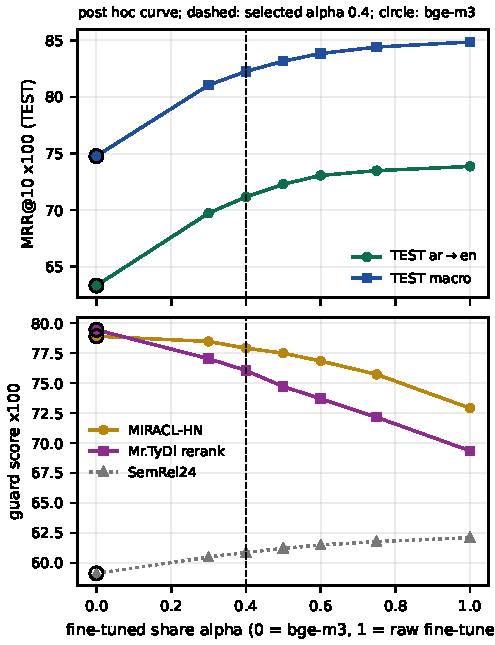
\includegraphics[width=\columnwidth]{figures/alpha_curve.pdf}}{\fbox{\parbox{0.9\columnwidth}{\TODO{WiSE curve: results/retrieval\_v2/alpha\_curve.json pending; report/make\_figures.py draws it}}}}
\caption{WiSE trade-off (post hoc): fine-tuned share $\alpha$ against test \ardir{}, test macro and the guard tasks; the circle is bge-m3, the dashed line the selected $\alpha$.}\label{fig:alpha}
\end{figure}

\subsection{MTEB(ara, v1) and its uncertainty}
bge-m3 leads the leaderboard at \NumMtebBgeTask{} mean over tasks, and the v1 fine-tune (\NumMtebVOneTask) ends below its own starting point, multilingual-E5-small: the cross-lingual gain was paid for on tasks unlike the training data, in particular Mr.TyDi re-ranking (\NumGuardESmallNamaa{} to \NumGuardVOneNamaa) and MIRACL (\NumGuardESmallMiracl{} to \NumGuardVOneMiracl).
With \NumMtebTasks{} tasks, differences of a point or two are within noise; Table~\ref{tab:paired} quantifies this with a bootstrap over tasks and an exact sign test.
v2-m3 and bge-m3 differ by \NumPairedMMeanDiff{} mean points (\NumCiLevel\% interval \NumPairedMCiLo{} to \NumPairedMCiHi), with \NumPairedMWins{} wins, \NumPairedMLosses{} losses and \NumPairedMTies{} tie over \NumPairedMTasks{} tasks (sign test $p$ = \NumPairedMSignP): the aggregate cannot separate them, because gains on retrieval tasks (largest: \NumPairedMBestTask, \NumPairedMBestGain) are offset by losses on MIRACL and Mr.TyDi re-ranking (largest: \NumPairedMWorstTask, \NumPairedMWorstGain).
On the Arabic$\leftrightarrow$English subsets alone, v2-m3 is ahead by \NumPairedMCrossDiff{} (\NumPairedMCrossCiLo{} to \NumPairedMCrossCiHi{}) with \NumPairedMCrossWins{} wins, \NumPairedMCrossLosses{} losses and \NumPairedMCrossTies{} tie over \NumPairedMCrossTasks{} tasks (sign test $p$ = \NumPairedMCrossP), consistent with the gains on the held-out benchmark but based on very few tasks.
For scale, bge-m3 against multilingual-E5-base differs by \NumPairedRefMeanDiff{} (\NumPairedRefCiLo{} to \NumPairedRefCiHi{}, $p$ = \NumPairedRefSignP), so the benchmark does resolve gaps of that size.
Students against multilingual-E5-base: \NumPairedBMeanDiff{} (\NumPairedBCiLo{} to \NumPairedBCiHi{}).

\begin{table*}[t]
\centering\tabfont
\begin{tabular}{@{}lrrrrrrrr@{}}
\toprule
Model & Task & Type & Retr. & Rerank & STS & Cls. & ar & ar-en \\
\midrule
bge-m3 & 72.0 & 70.9 & 73.5 & 79.4 & 66.3 & 64.5 & 70.4 & 73.3 \\
multilingual-e5-large & 71.4 & 70.3 & 74.0 & 79.6 & 68.1 & 61.8 & 69.5 & 75.3 \\
multilingual-e5-base & 67.9 & 67.3 & 68.8 & 77.1 & 64.9 & 59.6 & 66.5 & 69.1 \\
multilingual-e5-small & 65.6 & 65.7 & 66.0 & 79.2 & 60.1 & 58.3 & 65.0 & 63.9 \\
arabic-english-e5-small-retrieval & 65.0 & 64.4 & 66.3 & 65.9 & 57.4 & 59.0 & 63.1 & 68.1 \\
paraphrase-multilingual-MiniLM-L12-v2 & 58.7 & 62.7 & 45.2 & 70.0 & 63.1 & 52.0 & 54.6 & 66.5 \\
silma-embeddding-matryoshka-v0.1 & 60.3 & 61.9 & 47.1 & 71.4 & 59.2 & 63.2 & 62.2 & 47.9 \\
LaBSE & 58.2 & 58.7 & 46.2 & 51.6 & 62.5 & 58.3 & 54.2 & 66.2 \\
Arabic-Retrieval-v1.0 & 58.3 & 56.8 & 55.8 & 65.2 & 62.8 & 64.0 & 67.4 & 27.9 \\
Arabic-Triplet-Matryoshka-V2 & 55.7 & 54.8 & 51.0 & 64.5 & 60.3 & 63.4 & 66.3 & 19.5 \\
\midrule
v2-small & \TODO{pending} &  &  &  &  &  &  &  \\
v2-base & \TODO{pending} &  &  &  &  &  &  &  \\
v2-m3 & \TODO{pending} &  &  &  &  &  &  &  \\
\bottomrule
\end{tabular}

\caption{MTEB(ara, v1), scores $\times100$. Task = mean over tasks, Type = mean over task types; ar / ar-en = mean over Arabic-only / Arabic--English subsets. v2 rows are recomputed from the per-task scores of the paired comparison.}\label{tab:mteb}
\end{table*}

\begin{table}[t]
\centering\tabfont
\adjustbox{max width=\columnwidth}{\begin{tabular}{@{}lrrcrr@{}}
\toprule
Mean (Task) difference, new $-$ ref & tasks & diff & \NumCiLevel\% CI (tasks) & W/L/T & sign p \\
\midrule
first candidate (WiSE $\alpha{=}0.75$) vs bge-m3 & 19 & +0.06 & [$-$1.14, +1.16] & 9/9/1 & 1.00 \\
v2-m3 vs bge-m3 & 19 & +0.31 & [$-$0.34, +0.93] & 10/8/1 & 0.81 \\
\quad ar-en cross-lingual subsets & 6 & +1.73 & [+0.73, +2.77] & 5/0/1 & 0.06 \\
\quad ar-only subsets & 17 & +0.09 & [$-$0.55, +0.69] & 9/8/0 & 1.00 \\
v2-m3 seed 16 vs bge-m3 & 19 & +0.30 & [$-$0.40, +0.95] & 10/8/1 & 0.81 \\
v2-m3 seed 17 vs bge-m3 & 19 & +0.29 & [$-$0.39, +0.91] & 10/7/2 & 0.63 \\
v2-base vs mE5-base & 19 & +1.02 & [$-$0.52, +2.37] & 15/4/0 & 0.02 \\
\quad ar-en cross-lingual subsets & 6 & +5.14 & [+2.75, +7.41] & 6/0/0 & 0.03 \\
\quad ar-only subsets & 17 & $-$0.15 & [$-$1.59, +1.13] & 10/7/0 & 0.63 \\
v2-small vs mE5-small & 19 & +0.57 & [$-$1.24, +2.19] & 11/8/0 & 0.65 \\
\quad ar-en cross-lingual subsets & 6 & +5.87 & [+3.43, +7.94] & 6/0/0 & 0.03 \\
\quad ar-only subsets & 17 & $-$0.92 & [$-$2.57, +0.51] & 6/11/0 & 0.33 \\
v2-small vs v1 & 19 & +1.19 & [+0.43, +1.92] & 15/4/0 & 0.02 \\
\quad ar-en cross-lingual subsets & 6 & +1.65 & [+0.90, +2.49] & 6/0/0 & 0.03 \\
\quad ar-only subsets & 17 & +1.04 & [+0.19, +1.84] & 13/4/0 & 0.05 \\
\midrule
\multicolumn{6}{@{}l}{\emph{reference pairs from the leaderboard of baseline models}} \\
bge-m3 vs mE5-base & 19 & +4.09 & [+2.83, +5.45] & 17/2/0 & 0.001 \\
mE5-base vs mE5-small & 19 & +2.26 & [+0.92, +3.71] & 14/5/0 & 0.06 \\
v1 vs mE5-small & 19 & $-$0.62 & [$-$2.91, +1.40] & 10/9/0 & 1.00 \\
bge-m3 vs mE5-large & 19 & +0.54 & [$-$0.51, +1.59] & 11/8/0 & 0.65 \\
\bottomrule
\end{tabular}
}
\caption{Paired uncertainty of MTEB(ara) mean differences: bootstrap over tasks, wins / losses / ties, exact two-sided sign test. The lower block compares models of the \NumMtebModels-model leaderboard, for scale.}\label{tab:paired}
\end{table}

\subsection{Guard tasks and the contamination analysis}
Table~\ref{tab:guards} reports three guard tasks in the MTEB protocol.
Relative to bge-m3, v2-m3 is \NumGuardSemRelGap{} points on SemRel24, but \NumGuardMiraclGap{} on MIRACL-HardNegatives (\NumGuardVTwoMMiracl{} vs \NumGuardBgeMiracl) and \NumGuardNamaaGap{} on Mr.TyDi re-ranking.
Our bar was to stay within \NumGuardBar{} point of bge-m3 on MIRACL while keeping test \ardir{} at \NumGuardBarArEn{} or above; it is \emph{not met}, and neither replay nor preservation closed the gap.
Contamination does not explain the gap away: splitting the queries into near-duplicates of TyDi-ar or MIRACL-ar training questions and the rest (Table~\ref{tab:clean}), the difference between v2-m3 and bge-m3 on the clean MIRACL queries is \NumCleanGapMiracl{} points (all queries: \NumAllGapSplitMiracl).
Only \NumMiraclCleanN{} MIRACL queries are clean, so the interval is wide, and the split used a slightly different scoring input than the MTEB protocol. \TodoCleanProtocol{}
bge-m3 lists MIRACL and Mr.TyDi among its training sets, so its absolute MIRACL number is not a clean reference either.

\begin{table}[t]
\centering\tabfont
\adjustbox{max width=\columnwidth}{\begin{tabular}{@{}lrrr@{}}
\toprule
Model & MIRACL-HN & Mr.TyDi rerank & SemRel24 \\
\midrule
mE5-small & 72.4 & 79.2 & 51.0 \\
v1 & 66.3 & 65.9 & 41.2 \\
mE5-base & 73.0 & 77.1 & 59.2 \\
bge-m3 & 78.9 & 79.4 & 59.1 \\
v2-small & 68.3 & 68.9 & 46.1 \\
v2-base & 70.7 & 68.2 & 59.0 \\
v2-m3 & 77.9 & 76.0 & 60.9 \\
\midrule
v2-m3 $-$ bge-m3 & $-$1.0 & $-$3.4 & +1.8 \\
v2-base $-$ mE5-base & $-$2.3 & $-$8.9 & $-$0.2 \\
v2-small $-$ mE5-small & $-$4.1 & $-$10.4 & $-$4.8 \\
\bottomrule
\end{tabular}
}
\caption{Guard tasks (MTEB protocol, $\times100$): MIRACL-HardNegatives (nDCG@10), Mr.TyDi re-ranking (MAP), SemRel24 (Spearman). These runs use slightly different numerics than Table~\ref{tab:mteb} (differences up to \NumGuardVsLeaderboardMax{} points for the same model and task).}\label{tab:guards}
\end{table}

\begin{table*}[t]
\centering\tabfont
\begin{tabular}{@{}lrrrrrr@{}}
\toprule
 & \multicolumn{3}{c}{MIRACL-HN ar (n=105+895)} & \multicolumn{3}{c}{Mr.TyDi rerank (n=891+27)} \\
Model & all & clean & flagged & all & clean & flagged \\
\midrule
bge-m3 & 79.0 & 71.9 & 79.9 & 79.4 & 79.1 & 88.5 \\
mE5-base & 73.0 & 67.4 & 73.6 & 77.4 & 77.2 & 82.7 \\
mE5-small & 72.4 & 64.7 & 73.3 & 79.3 & 79.2 & 84.1 \\
v1 & 65.8 & 54.0 & 67.2 & 65.8 & 65.6 & 70.7 \\
v2-m3 raw FT & 72.9 & 63.3 & 74.0 & 69.4 & 69.4 & 69.6 \\
v2-m3 & 77.9 & 70.5 & 78.8 & 76.0 & 75.9 & 80.7 \\
v2-base & 70.7 & 61.6 & 71.8 & 68.1 & 68.2 & 67.4 \\
v2-small & 68.3 & 57.1 & 69.6 & 68.9 & 68.7 & 74.2 \\
\bottomrule
\end{tabular}

\caption{Guard tasks split by contamination: ``clean'' queries are not near-duplicates of any TyDi-ar or MIRACL-ar training question, ``contam.'' queries are. Per-query scores in the contamination-split protocol.}\label{tab:clean}
\end{table*}

\subsection{Confirmatory seeds}
The model-selection experiments above used the first three seeds and several amended selection rules, so their headline numbers are exploratory (Table~\ref{tab:seeds}).
Two further seeds (\NumConfSeeds) were trained after the recipe was frozen (\TODO{freeze timestamp: quote from RESULTS\_v2.md}); Table~\ref{tab:confirm} is the confirmatory result.
Their mean \ardir{} is \NumConfArEnMean{} (macro \NumConfMacroMean{}), \NumConfDeltaArEn{} and \NumConfDeltaMacro{} points relative to bge-m3.

\begin{table}[t]
\centering\tabfont
\adjustbox{max width=\columnwidth}{\begin{tabular}{@{}lrr@{}}
\toprule
TEST, mean $\pm$ s.d. over three development seeds & ar$\to$en & macro \\
\midrule
raw fine-tune ($\alpha{=}1$) & 73.3 $\pm$ 0.6 & 84.5 $\pm$ 0.3 \\
v2-m3 recipe (WiSE) & 70.9 $\pm$ 0.3 & 82.2 $\pm$ 0.1 \\
v2-base students & 65.9 $\pm$ 0.2 & 79.9 $\pm$ 0.1 \\
v2-small students & 59.3 $\pm$ 0.3 & 76.8 $\pm$ 0.0 \\
\bottomrule
\end{tabular}
}
\caption{Exploratory seeds of the raw fine-tune (test); pending runs are marked.}\label{tab:seeds}
\end{table}

\begin{table}[t]
\centering\tabfont
\adjustbox{max width=\columnwidth}{\begin{tabular}{@{}lrrrr@{}}
\toprule
Model, seed & ar$\to$en & macro & $\Delta$ ar$\to$en vs bge-m3 & MTEB Mean (Task) \\
\midrule
v2-m3 recipe (WiSE), seed 16 & 71.1 & 82.2 & +7.7 [+6.6, +8.9] & 72.28 \\
v2-m3 recipe (WiSE), seed 17 & 70.3 & 82.0 & +7.0 [+5.8, +8.1] & 72.27 \\
v2-m3 recipe (WiSE), mean of 2 seeds & 70.7 & 82.1 & +7.3 [+6.2, +8.4] & 72.27 \\
\midrule
raw fine-tune ($\alpha{=}1$), seed 16 & 73.6 & 84.7 & +10.2 [+8.7, +11.8] & -- \\
raw fine-tune ($\alpha{=}1$), seed 17 & 73.1 & 84.3 & +9.8 [+8.2, +11.3] & -- \\
raw fine-tune ($\alpha{=}1$), mean of 2 seeds & 73.4 & 84.5 & +10.0 [+8.5, +11.4] & -- \\
\bottomrule
\end{tabular}
}
\caption{Confirmatory seeds, trained after the recipe was frozen (test). Intervals: paired bootstrap over queries against bge-m3.}\label{tab:confirm}
\end{table}

\section{Deployment Costs}\label{sec:deploy}
We export v2-small and v2-base to ONNX (fp32, opset \NumOpset, pooling and normalisation inside the graph) and compare three ways of shrinking them for CPU serving:
ONNX Runtime dynamic int8 with per-tensor or per-channel weight scales \citep[activations quantised on the fly, cf.][]{zafrir2019q8bert}, and weight-only 8-bit block quantisation of the MatMul weights that leaves the activations in fp32.
Quality is measured as MRR@10 on the same test split against the PyTorch fp32 model, on CPU, with paired bootstrap intervals.
Latency was measured on the \NumSparkCpus-core ARM CPU of a shared server (not an x86 laptop or cloud VM), one process, \NumThreadsLow{} and \NumThreadsHigh{} threads; numbers are therefore indicative.

Table~\ref{tab:deploy} shows that the ONNX fp32 graphs reproduce the PyTorch results (\NumDeltaOnnxSmall{} and \NumDeltaOnnxBase{} macro points) and cut single-query latency (\NumThreadsLow{} threads) from \NumQLatSmallTorch{} to \NumQLatSmallOnnx{} ms for v2-small and from \NumQLatBaseTorch{} to \NumQLatBaseOnnx{} ms for v2-base.
Dynamic int8 with per-tensor scales is faster still (\NumQLatSmallDyn{} and \NumQLatBaseDyn{} ms) but \emph{not acceptable} here: \NumDeltaDynSmall{} macro points for v2-small and \NumDeltaDynBase{} for v2-base (\NumDeltaDynBaseArEn{} on \ardir{} for the base model).
Per-channel scales reduce the loss to \NumDeltaPcSmall{} and \NumDeltaPcBase{}, still more than we would ship for the base model.
Weight-only 8-bit quantisation is lossless within noise (\NumDeltaWoSmall{} and \NumDeltaWoBase{}) and shrinks the models from \NumSizeSmallOnnx{} to \NumSizeSmallWo{} MiB and from \NumSizeBaseOnnx{} to \NumSizeBaseWo{} MiB, but its CPU kernels are slower per query than fp32 (\NumQLatSmallWo{} and \NumQLatBaseWo{} ms).
We therefore recommend ONNX fp32 when latency matters, weight-only 8-bit when download size matters, and no dynamic int8 for these models without calibration or quantisation-aware training.

\begin{table*}[t]
\centering\tabfont
\begin{tabular}{@{}lrrrrrrr@{}}
\toprule
Variant (CPU) & MiB & RSS & q@1 ms & p/s & MRR & $\Delta$ & $\Delta$ ar$\to$en \\
\midrule
v2-small PyTorch fp32 & 449 & 1813 & 21 & 13 & 77.0 & ref. & ref. \\
v2-small ONNX fp32 & 448 & 2600 & 14 & 13 & 77.0 & 0.00 & 0.00 \\
v2-small ONNX int8 & 113 & 2245 & 5 & 27 & 74.8 & $-$2.19 & $-$3.64 \\
v2-small ONNX int8, per-channel & 113 & 2255 & 5 & 25 & 76.3 & $-$0.65 & $-$1.49 \\
v2-small ONNX weight-only 8-bit (MatMulNBits) & 114 & 2269 & 24 & 14 & 76.9 & $-$0.01 & $-$0.01 \\
\midrule
v2-base PyTorch fp32 & 1061 & 2440 & 68 & 5 & 80.2 & ref. & ref. \\
v2-base ONNX fp32 & 1059 & 3093 & 49 & 6 & 80.2 & 0.00 & 0.00 \\
v2-base ONNX int8 & 265 & 2305 & 14 & 16 & 77.0 & $-$3.11 & $-$4.81 \\
v2-base ONNX int8, per-channel & 266 & 2302 & 14 & 26 & 77.7 & $-$2.41 & $-$4.37 \\
v2-base ONNX weight-only 8-bit (MatMulNBits) & 270 & 2225 & 86 & 4 & 80.1 & $-$0.02 & $-$0.12 \\
\bottomrule
\end{tabular}

\caption{CPU deployment variants. MiB: size on disk; RSS: peak resident memory of the benchmark process (\NumThreadsHigh{} threads; includes the python and data-loading baseline of that process); q@1: p50 latency of a single query (\NumThreadsLow{} threads, ms); p/s: passages per second (batch 32, \NumThreadsHigh{} threads); MRR: test macro MRR@10 $\times100$; $\Delta$: difference to PyTorch fp32 in points (macro, and \ardir{}).}\label{tab:deploy}
\end{table*}

\section{Data Card and Licences}
Table~\ref{tab:licences} lists every dataset and model used, how it entered the study, and the licence on its Hugging Face card (checked \NumLicChecked).
The final recipe trains on TyDi QA (\LicTydi), SQuAD v1.1 (\LicSquad) and ARCD (\LicArcd) and on machine translations of their questions produced by Gemma-4-26B-A4B (\LicGemma); the starting weights are bge-m3 (\LicBge) and multilingual-E5 (\LicEBase).
MIRACL Arabic (\LicMiracl) was used only in an ablation, XQuAD (\LicXquad) only for testing, and the remaining sources only for validation or selection.
Passage text is Wikipedia content, so share-alike terms of SQuAD and Wikipedia apply to derived corpora.
\TODO{licence of the released weights: author decision; the training data include CC BY-SA sources}

\begin{table*}[t]
\centering\tabfont
\begin{tabular}{@{}p{0.34\textwidth}p{0.22\textwidth}p{0.3\textwidth}@{}}
\toprule
Source & Role & Licence (Hub card) \\
\midrule
TyDi QA GoldP (Arabic, English) & training data (final recipe) & apache-2.0 \\
SQuAD v1.1 train & training data (final recipe) & cc-by-sa-4.0 \\
ARCD & training data (final recipe) & mit \\
XQuAD & evaluation / selection only & cc-by-sa-4.0 \\
MIRACL Arabic (queries, qrels, corpus) & training data (ablation only) & apache-2.0 \\
Gemma-4-26B-A4B (query translator) & translated the training queries & apache-2.0 \\
bge-m3 (base weights of v2-m3, teacher baseline) & initial weights & mit \\
multilingual-E5-base (base of v2-base) & initial weights & mit \\
multilingual-E5-small (base of v2-small) & initial weights & mit \\
ArSarcasm (selection suite) & evaluation / selection only & mit \\
XNLI (selection suite) & evaluation / selection only & no licence tag on the Hub card \\
Arabic STS-B (selection suite) & evaluation / selection only & apache-2.0 \\
mMARCO Arabic (selection proxy) & evaluation / selection only & no licence tag on the Hub card \\
\midrule
Weights of v2-m3, v2-base, v2-small & released models & \TODO{licence of the weights: author decision (training data include share-alike sources)} \\
\bottomrule
\end{tabular}

\caption{Data card: sources, roles and licences. ``No licence tag'' means the Hub card does not state one; nothing is assumed.}\label{tab:licences}
\end{table*}

\section{Limitations}
Most fine-tuned numbers are single seeds; the confirmatory seeds cover the final recipe only, and the WiSE blends and students of other seeds are pending (Tables~\ref{tab:seeds}, \ref{tab:confirm}).
The test set is Wikipedia-style extractive QA with \NumStyleN{} parallel questions per XQuAD direction, so the intervals are wide for the cross-lingual slices; dialects, informal text and long documents are untested.
Training queries are machine-translated and not human-verified; the offset check cannot rule out subtler translationese, and dev cross-lingual numbers are inflated by it.
The guard analysis shows a real regression on MIRACL and Mr.TyDi, and the clean subset is small.
MTEB(ara, v1) has \NumMtebTasks{} tasks and \NumMtebModels{} scored models; its aggregate cannot resolve differences of about a point (Table~\ref{tab:paired}).
The selection rules were amended during the work (Appendix~\ref{app:prereg}); the post-hoc WiSE curve and the exploratory seeds should not be read as confirmatory.
Deployment latency comes from one machine type, with other jobs running, and does not include serving overhead.
No RAG-level evaluation is done here.

\section{Reproducibility}
Every number in this report is generated by \texttt{report/make\_tables.py} from the committed result files in \texttt{results/retrieval\_v2}, \texttt{results/mteb\_ara} and \texttt{deploy/results}; the figure by \texttt{report/make\_figures.py};
run \texttt{make -C report pdf}. Training used a single GB10 GPU; the evaluation harness is in the accompanying repository and the deployment scripts are in \texttt{deploy/}.
The data are public (Table~\ref{tab:licences}); the v2 model weights are \TODO{published after review: Hugging Face repository names}.

{\small\setlength{\bibsep}{1pt}
\bibliography{refs}}

\appendix
\section{Pre-registration Trail}\label{app:prereg}
The selection of the v2-m3 recipe followed rules that were written down in the lab notebook of the training machine before the runs they govern.
Below, the notebook entries are quoted verbatim apart from LaTeX escaping, with their timestamps: the rule that fixed $\alpha$, the original replay/preservation rule, amendment 1 (a validation suite, written before any candidate was scored on it, with a same-day correction) and amendment 2 (an extended range of $\alpha$ and a rerun of the LoRA candidate after a bug in the first run).
The amendments changed the selection procedure after earlier selections had been made, which is why the confirmatory seeds and the post-hoc curve are reported separately.
\paragraph{WiSE alpha selection rule, as recorded in the results entry (2026-11-04 11:05)}
{\footnotesize\raggedright
Selection rule fixed BEFORE any guard eval: dev macro within 0.5 of raw AND proxy within 1.0 of bge-m3 $\to$ alpha 0.75.\par}

\paragraph{Original pre-registered rule (2026-11-04 14:00)}
{\footnotesize\raggedright
2026-11-04 \textasciitilde{}14:00 coordinator: fix the MIRACL forgetting properly (replay + preservation), PRE-REGISTERED selection rule

- Why: v2-m3 + WiSE a.75 scores MIRACL-HN.v2 75.7 vs bge-m3 79.0 (-3.3); bar = within 1 pt while TEST ar$\to$en >= 72.

- Replay data: MIRACL-ar TRAIN (miracl/miracl topics+qrels, miracl/miracl-corpus; Apache-2.0; judged-relevant = positives, judged-NOT-relevant = hard negatives), 500 queries HELD OUT as the selection-only slice devM (own mini-corpus of judged passages + 10k random distractors, evaluated separately, never in the dev macro). Filters: near-duplicate of any MIRACL-ar dev query / v1 test+dev query, positive overlapping a MIRACL dev positive or a v1 test passage; contam\_v2 then applies the whole MTEB(ara) list. Mr.TyDi-ar train: not added (its questions ARE the TyDi-ar train questions v1/v2 already use; script-based loader).

- Preservation loss: 1 - cos(student, frozen bge-m3) on Arabic positives, weight 0.5 (sweep not affordable: one m3 run = 55 min).

- Runs (seed 13, m3 recipe of m3\_b\_s13): m3\_r (replay), m3\_p (preservation), m3\_rp (both); each also WiSE a.75 / a.50 against bge-m3; evaluation = dev (4 directions), devM, mMARCO proxy. NO guard is used for selection.

- RULE (fixed now, before the runs): a candidate qualifies if (i) devM MRR@10 >= bge-m3's devM - 1.0, (ii) dev ar$\to$en >= 79.0 (\textasciitilde{} TEST 72), (iii) dev macro >= m3\_b dev macro (85.3) - 1.5; among qualifying take the highest dev macro (ties: fewer moving parts). If none qualifies: highest devM among those with dev ar$\to$en >= 79.0, reported as a miss.

- Seed 14 of the OLD recipe is allowed to finish (running); seed 15 is NOT run with the old recipe. KD ablations/baseline guards are queued after these runs.\par}

\paragraph{Amendment 1: validation-suite selection (2026-11-04 19:05)}
{\footnotesize\raggedright
2026-11-04 \textasciitilde{}19:05 - PRE-REGISTRATION: validation suite for the final v2-m3 pick (written BEFORE any candidate is scored on the new components)

Trigger: coordinator, "0.06 is a tie; the losses (Namaa, MIRACL, XNLI, AJGT) are drift away from bge-m3's general skills; select on a validation suite that mirrors the MTEB(ara)

task types, never on MTEB". Supersedes select\_m3.py (kept as the record of the earlier rule). No MTEB(ara) number and no TEST number is read by this procedure.

Order of work: s15 $\to$ soup/blends $\to$ suite (interim table) $\to$ LoRA / freeze $\to$ suite (all) $\to$ selection $\to$ ONE MTEB(ara) scoring of the pick $\to$ teacher = pick $\to$ students.

DEVIATION FROM THE BRIEF (flagged to the coordinator): the brief asks for the XNLI-ar VALIDATION split "since MTEB uses test". mteb's XNLI task sets

eval\_splits=["test","validation"] (pylibs/mteb/tasks/pair\_classification/multilingual/xnli.py) and the leaderboard number is the mean over both, so the validation split is

part of the MTEB evaluation. Instead: a seeded 3,000-pair subsample of the XNLI-ar TRAIN split (facebook/xnli, ar/train; machine-translated MNLI; entailment=1,

contradiction=0, neutral dropped, as mteb does). Never trained on, never part of any MTEB split.

COMPONENTS (6, all x100, higher = better):

1 dev      : v2 extended DEV macro MRR@10 over the 4 directions (ar$\to$en, en$\to$ar, ar$\to$ar, en$\to$en)            [results/NAME.dev.json]

2 devM     : MIRACL-ar TRAIN hold-out (500 queries, selection-only slice, excluded from training), MRR@10                [NAME.devM.json]

3 proxy    : mMARCO-ar dev proxy (1,000 q / 25k docs, seed 13), MRR@10                                                    [results/ood\_dev\_ar.json]

4 xnli     : average precision of the cosine similarity on 3,000 XNLI-ar TRAIN pairs (seed 13)                            [results/suite/NAME.json]

5 cls      : mean of two 8-shot-per-label logistic-regression probes (mteb protocol: 10 experiments, samples\_per\_label=8, max\_iter=100) on ArSarcasm

(iabufarha/ar\_sarcasm, licence MIT): (a) sarcasm 2-class, (b) sentiment 3-class. The probe is fitted on rows of the TRAIN split and scored on

2,000 other TRAIN rows (seeded hold-out). MTEB scores TweetSarcasmClassification on the ar\_sarcasm TEST split; the TRAIN split is disjoint

from it (same source, so it is a close proxy by design). AJGT / TweetEmotion / HotelReview are not touched.

6 sts      : Spearman of cosine similarity on the Arabic DEV split of stsb\_multi\_mt (PhilipMay/stsb\_multi\_mt, ar/dev, 1,500 pairs; machine-translated STSb; licence

"other" - used for validation only, not redistributed). Disjoint from STS17 / STS22 / SemRel24 (the MTEB STS tasks).

NORMALISATION: per component c, x\_c is min-max scaled over the POOL = \{all candidates + the reference rows (bge-m3, m3\_b\_s13 raw, soup raw)\}:

n\_c = (x\_c - min\_pool) / max(max\_pool - min\_pool, 1.0 point)     (the 1-point floor keeps a component whose pool range is below the noise level from being inflated)

SCORE = unweighted mean of the 6 n\_c. Reported with the 6 raw components.

POOL / CANDIDATES (selectable): WiSE alpha in \{0.4,0.5,0.6,0.75\} of m3\_b\_s13 (wm\_a50, wm\_a75 exist; w\_m3b\_a40, w\_m3b\_a60 new);

SOUP = uniform average of the seed 13/14/15 fine-tunes (m3\_b\_s13/s14/s15; seed 15 is trained first), then WiSE alpha in \{0.4,0.5,0.6,0.75\} (soup\_a40..a75);

LoRA r=32 attention+MLP lr 1e-4 (m3\_lo\_s13) and freeze-bottom-12 (m3\_fr\_s13) raw, plus their WiSE blends alpha \{0.75,0.5\}.  14 selectable models.

Reference rows (in the pool for normalisation, shown, NOT selectable): bge-m3, m3\_b\_s13 raw (alpha=1), soup raw.

ELIGIBILITY (protects the S\_TIER ar$\to$en bar): dev ar$\to$en >= bge-m3 dev ar$\to$en + 5.0 points.

PICK = the eligible candidate with the highest SCORE.  Ties (|diff| < 0.02) $\to$ fewer ingredients: single-seed WiSE < soup WiSE < LoRA/freeze (then larger alpha).

The pick is announced here before its MTEB(ara) scoring; that scoring is run once and reported even if it is lower than final\_m3\_wa75\_s13 (72.044). Earlier MTEB(ara)

scoring of final\_m3\_wa75\_s13 happened BEFORE this suite existed and is not used in the selection.

3-SEED REPORTING: pick is a soup $\to$ the soup is the reported model (one model; paired bootstrap over queries); otherwise the per-seed blends (13/14/15) of the picked recipe.

Students: distilled from the FINAL teacher (the pick), KD-only; teacher embeddings are recomputed from the pick (tag m3f).

Code: lab/retrieval/v2/suite\_v2.py (components 4-6), suite\_select.py (assembly + rule), runs/retrieval/v2/scripts/drive14.sh (queue).

- 2026-11-04 \textasciitilde{}19:20 CORRECTION to the pre-registration above (still before any candidate has a suite number): PhilipMay/stsb\_multi\_mt has NO Arabic split (checked on the Hub),

so component 6 uses the Arabic STS-B VALIDATION split of Omartificial-Intelligence-Space/Arabic-stsb (apache-2.0; machine-translated STS-B, 1,500 pairs; validation.csv, "score" column).

Everything else is unchanged. Data fetched to runs/retrieval/v2/data/suite/ (xnli\_ar\_train.parquet, ar\_sarcasm\_train.parquet, stsb\_ar\_validation.csv).\par}

\paragraph{Amendment 2: alpha extension and LoRA rerun (2026-11-04 21:35)}
{\footnotesize\raggedright
2026-11-04 \textasciitilde{}21:35 - AMENDMENT 2 to the pre-registered suite selection (coordinator follow-up after DRIVE14\_DONE); written BEFORE any of the runs below

What happened in drive14 (facts, from the logs; the "rc=0" lines of the driver are NOT reliable because run\_docker.sh masks the exit code - from now on every step is verified by the existence of its output file):

* LoRA: m3\_lo\_s13 trained all 615/615 steps (56 min) and then CRASHED in train\_v2.py at merge\_and\_unload (AttributeError: 'XLMRobertaModel' has no attribute 'merge\_and\_unload'): my code

kept the in-place-injected XLM-R module instead of the PeftModel handle. Nothing was saved (the adapters died with the process), so the LoRA dev / merges / blends / proxy2 / suite2 all failed on the missing path

within seconds. This is a bug in MY code, not a result about LoRA.  proxy2 and suite2 aborted at their FIRST model (LoRA), so the freeze run and its two blends (which trained fine: dev 85.0 / 84.8 / ..., devM 78.8 / 79.7 / ...) have no proxy and suite numbers.

* select2's "PICK (interim)" was computed on the 11 complete models only.

* Tie rule: the pre-registration says "|diff| < 0.02" (strict). select code used >= best - 0.02 (inclusive). Corrected to strict; exact differences are printed to 4 decimals; the pick report states which clause decided.

DECISIONS (no re-litigation after this entry):

A. LoRA is RERUN with the identical recipe / seed (m3\_lo\_s13, r=32, lr 1e-4, attention+MLP, 1 epoch, seed 13) after a gated 3-minute merge self-test of the fixed code (adapter saved to disk before the merge). \textasciitilde{}57 min. Reason: it is the only

pre-registered candidate that constrains the update DURING training (freeze did not help on devM); the GPU would otherwise idle until the pick. It enters the pool exactly as registered (raw + WiSE .75 / .5).

B. Order: (1) freeze proxy + suite  $\to$  (2) select on the pool WITHOUT LoRA $\to$ winning family F by the rule as written (strict tie)  $\to$  (3) ONE extra pair of alphas for F ONLY: alpha 0.30; alpha 0.35 is added ONLY if the

0.30 model fails eligibility (dev ar$\to$en < 78.5 = bge-m3 dev ar$\to$en 73.5 + 5.0); if 0.30 is eligible, 0.35 is NOT run; nothing below 0.30 is tried  $\to$  (4) LoRA rerun + blends  $\to$  (5) FINAL select on the FULL pool

(all earlier candidates + the 0.30/0.35 point(s) + LoRA models), same normalisation (pool-wide min-max, 1-point floor), same eligibility, same strict tie rule  $\to$  (6) ONE MTEB(ara) scoring of that pick (= final\_m3), reported even if lower.

If LoRA wins the final select there is no further alpha extension. The alphas 0.30 / 0.35 are selectable. Family names for the extension: wise $\to$ w\_m3b\_a30 / a35; soup $\to$ soup\_a30 / a35; freeze $\to$ w\_m3\_fr\_s13\_a30 / a35.

C. Everything else in the first pre-registration (components, normalisation, eligibility, tie-break by ingredients, 3-seed reporting) is unchanged. No MTEB(ara) and no TEST number is read by any of the selection steps.\par}


\end{document}
